\section*{Arreglos unidimencionales}

%- - - - - - - - - - - - - - - - - Título - - - - - - - - - - - - - - - - - -%
\begin{frame}[c] 
\centering
\huge \textbf{Arreglos unidimencionales}
\end{frame}

% - - - - - - - - - - - - - - - - - - - - Slide01 - - - - - - - - - - - - - - - - -
\begin{frame}
    \frametitle{Arreglos Unidimencionales}
    \framesubtitle{Definición e Inicialización}
    \begin{center}
        \textbf{Definición}
    \end{center}
    \justify
    \hspace{5mm}Un arreglo es un tipo de dato estructurado que almacena en una sola variable un conjunto limitado de elementos del mismo tipo. El nombre del arreglo apunta a la dirección del primer elemento del arreglo. Los datos se llaman elementos del arreglo y su posición se numera consecutivamente: 1, 2, 3…n. Un arreglo inicia en la posición cero, por lo tanto el i-ésimo elemento está en la posición i-1, es decir si el arreglo llamado \textbf{a} tiene \textbf{\textit{n}} elementos, sus nombres son a[0], a[1], ..., a[n-1].\\
\end{frame}


% - - - - - - - - - - - - - - - - - - - - Slide02 - - - - - - - - - - - - - - - - -
\begin{frame}
\frametitle{Arreglos Unidimencionales}
\framesubtitle{Definición e Inicialización}
    \justify
    Para acceder a un elemento específico de un arreglo se usa un índice o subíndice.
    Un arreglo se caracteriza por:
    \begin{enumerate}
        \item Ser una lista de un número finito de n elementos del mismo tipo.
        \item Almacenar los elementos del arreglo en memoria contigua.
        \item Tener un único nombre de variable que representa a todos los elementos y éstos se diferencian por un índice o subíndice.
        \item Acceder de manera directa o aleatoria a los elementos individuales del arreglo, por el nombre del arreglo y el índice o subíndice.
    \end{enumerate}
\end{frame}


% - - - - - - - - - - - - - - - - - - - - Slide03 - - - - - - - - - - - - - - - - -
\begin{frame}[fragile]
    \frametitle{Arreglos Unidimencionales}
    \framesubtitle{Definición e Inicialización}
    Formato para declarar un arreglo unidimencional.
    \vspace{2mm}
    \begin{lstlisting}
        tipoDato identifArreglo[tamArreglo];
\end{lstlisting}
Donde:
\begin{itemize}
    \item \textbf{tipoDato} se refiere al tipo de dato de cada elemento del arreglo; puede ser entero, real, carácter, etcétera. \pause
    \item \textbf{identifArreglo} es el nombre que representa a todo el arreglo.\pause
    \item \textbf{tamArreglo} es la cantidad de elementos que contiene el arreglo.\pause
\end{itemize}
\end{frame}


% - - - - - - - - - - - - - - - - - - - - Slide04 - - - - - - - - - - - - - - - - -
\begin{frame}[fragile, t]
    \frametitle{Arreglos Unidimencionales}
    \framesubtitle{Definición e Inicialización}
    \begin{center}\textbf{Ejemplo}\end{center}
        \vspace{-4mm}
    \begin{lstlisting}
float x[8];
    \end{lstlisting}
    \vspace{-5mm}
\begin{center}
        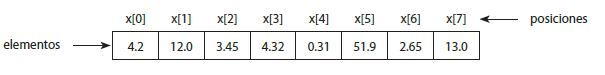
\includegraphics[scale=0.55]{figs/ejemploArregloUnidimencional}
\end{center}
\vspace{-6mm}
\justify
\hspace{5mm}Este arreglo contiene ocho elementos almacenados entre la posición (0-7). Para referirnos a un elemento en particular dentro del arreglo, especificamos el nombre del arreglo y el número de posición donde se encuentra ubicado. La posición del arreglo va entre corchetes (“[ ]”).
\end{frame}


% - - - - - - - - - - - - - - - - - - - - Slide05 - - - - - - - - - - - - - - - - -
\begin{frame}[fragile]
    \frametitle{Arreglos Unidimencionales}
    \framesubtitle{Definición e Inicialización}
    Si la instrucción fuera imprimir \textbf{x[4]} se mostrará el valor de 0.31\\
    \begin{lstlisting}
printf("%f", x[4]);
    \end{lstlisting}
    Para almacenar la suma de los valores contenidos en los primeros tres elementos del arreglo x, escribiríamos:\\
    \begin{lstlisting}
a = x[0] + x[1] + x[2];
printf("%f", a);
    \end{lstlisting}
    Para dividir el valor del séptimo elemento del arreglo x entre 2 y asignar el resultado a la variable c escribiríamos:
    \begin{lstlisting}
c = x[6]/2;
    \end{lstlisting}
\end{frame}

% - - - - - - - - - - - - - - - - - - - - Slide06 - - - - - - - - - - - - - - - - -
\begin{frame}[fragile,t]
    \frametitle{Arreglos Unidimencionales}
    \framesubtitle{Definición e Inicialización}
    \begin{center}
        \textbf{Inicialización}
    \end{center}
    En el momento de declarar el arreglo, se especifican los valores.
    \begin{lstlisting}
/*tipoDato identif[tamArreglo]={valores};*/
int lista[5] = {10,17,8,4,9};
    \end{lstlisting}
    \vspace{-3mm}
    Para llenar un arreglo completo se utiliza generalmente el ciclo desde \textbf{(for}) facilitando con la variable de control el incremento de la \textbf{\textit{i}}, donde la \textbf{\textit{i}} representa el subíndice.
    \begin{lstlisting}
for(i=0;i<5;i++)
    printf("%d", lista[i]);
    \end{lstlisting}
\end{frame}


% - - - - - - - - - - - - - - - - - - - - Slide07 - - - - - - - - - - - - - - - - -
\begin{frame}[fragile]
    \frametitle{Arreglos Unidimencionales}
    \framesubtitle{Definición e Inicialización}
    \begin{center}
        \textbf{Modificación}
    \end{center}
    \justify
    Para modificar los elementos de un vector en cualquier momento, sólo es necesario especificar el nombre del arreglo unidimensional, la posición y el nuevo valor. Enseguida se muestra la sintaxis a seguir:
    \begin{lstlisting}
/*tipoDato identArr[pos]=valor;*/
int b[3] = 18;
    \end{lstlisting}
    Donde \textbf{valor} es un dato, el resultado de alguna operación lógica o aritmética, etc.
\end{frame}